% !TeX program = xelatex
\documentclass[aspectratio=169, 12pt, xcolor=table]{beamer}

% ============== PACKAGES ==============
\usepackage{fontspec}
\usepackage{polyglossia}
\setdefaultlanguage{vietnamese}
\usepackage{amsmath, amssymb}
\usepackage{graphicx}
\usepackage{booktabs}
\usepackage{tikz}
\usetikzlibrary{arrows, calc, positioning, backgrounds}
\usepackage{appendixnumberbeamer}

% ============== THEME ==============
\usetheme{SimplePlus}
\definecolor{UTHblue}{RGB}{0, 51, 102}
\definecolor{UTHgold}{RGB}{255, 183, 27}

% ============== METADATA ==============
\title[Offline RL Gas Optimization]{Ứng dụng Offline Reinforcement Learning\\Tối ưu Chi phí Gas trên Ethereum}
\author[Duy, Long, Thảo, Hà, Dung, Khiêm]{
  \footnotesize
  Nguyễn Tiến Duy (079205037141) \quad Nguyễn Thành Long (022205011246) \\
  Đỗ Nguyễn Phương thảo (036305007143) \quad Hoàng Lê Việt Hà (04430511246) \\
  Trần Thảo Dung (079305007143) \quad Võ Trần Khiêm (052205007100)
}
\institute[UTH]{
  Trường Đại học Giao thông Vận tải TP.HCM\\
  Viện Công nghệ Thông tin và Điện, Điện tử\\[0.3em]
  \textbf{GVHD:} TS. Nguyễn Thị Khánh Tiên
}
\date{Tháng 05/2026}

\begin{document}

% =====================================================================
% SLIDE 1: TITLE
% =====================================================================
\begin{frame}[plain]
  \titlepage
\end{frame}

% =====================================================================
% SLIDE 2: OUTLINE
% =====================================================================
\begin{frame}{Nội dung trình bày}
  \tableofcontents
\end{frame}

% =====================================================================
% PHẦN 1: BÀI TOÁN
% =====================================================================
\section{Bài toán}

\begin{frame}{Bối cảnh: Chi phí Gas trên Ethereum}
  \begin{columns}[T]
    \begin{column}{0.55\textwidth}
      \begin{itemize}
        \item Mỗi giao dịch trên Ethereum phải trả \textbf{Gas Fee}
        \item Phí dao động liên tục theo mức độ tắc nghẽn mạng
        \item Giờ cao điểm: phí tăng \textbf{gấp 5--10 lần}
        \item[\(\Rightarrow\)] \textbf{Bài toán Timing:} Khi nào gửi giao dịch để tiết kiệm nhất?
      \end{itemize}
      \vspace{1em}
      \begin{block}{Ràng buộc}
        Tất cả giao dịch phải hoàn tất trước \textbf{Deadline 24h}\\
        (\textbf{0\% Miss Rate} — Zero-Miss SLA)
      \end{block}
    \end{column}
    \begin{column}{0.42\textwidth}
      
\includegraphics[width=\textwidth]{Images/04_episode_snapshot.png}
    \end{column}
  \end{columns}
\end{frame}

\begin{frame}{Mô hình hóa: Markov Decision Process}
  \begin{block}{Phát biểu bài toán}
    Tại mỗi block $t$, hệ thống quyết định số lượng giao dịch cần gửi để
    \textbf{tối thiểu tổng Gas Cost} mà vẫn đảm bảo \textbf{Deadline}.
  \end{block}
  \vspace{0.5em}
  \begin{columns}[T]
    \begin{column}{0.48\textwidth}
      \textbf{State} $s_t \in \mathbb{R}^{11}$:
      \begin{itemize}
        \item Giá gas: $g_t, g_{t-1}, g_{t-2}$
        \item Tắc nghẽn: $p_t$, Momentum: $m_t$
        \item Queue: $Q_t$, Deadline: $\tau_t$
        \item Backlog Pressure: $b_t$ (AR model)
      \end{itemize}
    \end{column}
    \begin{column}{0.48\textwidth}
      \textbf{Action} $a_t \in \{0,1,2,3,4\}$:
      \begin{itemize}
        \item Bin 0: Giữ hàng (0\%)
        \item Bin 1--3: Xả 25\%, 50\%, 75\%
        \item Bin 4: Xả 100\%
      \end{itemize}
      \vspace{0.5em}
      \textbf{Reward:}
      \begin{itemize}
        \item Gas cost (âm)
        \item Urgency penalty (hàm mũ)
        \item Deadline penalty
      \end{itemize}
    \end{column}
  \end{columns}
\end{frame}

% =====================================================================
% PHẦN 2: PHƯƠNG PHÁP
% =====================================================================
\section{Phương pháp}

\begin{frame}{Hindsight Oracle — Bộ Giải Tối ưu Toàn cục}
  \begin{columns}[T]
    \begin{column}{0.55\textwidth}
      \begin{itemize}
        \item \textbf{Vấn đề:} Dataset thô chứa hành vi suboptimal
        \item \textbf{Giải pháp:} Xây dựng \textbf{DP Solver toàn tri}
        \item Biết trước giá gas 24h $\Rightarrow$ tối ưu toàn cục
        \item Tạo ra \textbf{quỹ đạo chuyên gia} làm nhãn huấn luyện
      \end{itemize}
      \vspace{0.5em}
      \begin{block}{Backward Pass}
        $V[t,Q] = \min_{b\in\mathcal{A}} \{c(t,Q,b) + V[t+1, f(Q,b,t)]\}$
      \end{block}
    \end{column}
    \begin{column}{0.42\textwidth}
      \begin{tikzpicture}[
        box/.style={rectangle, draw, rounded corners, fill=UTHblue!10,
          minimum width=2cm, minimum height=0.6cm, text centered, font=\scriptsize},
        arrow/.style={->, thick, UTHblue}
      ]
        \node[box] (raw) at (0,0) {Raw Parquet};
        \node[box] (feat) at (0,-1) {Feature Eng.};
        \node[box] (oracle) at (0,-2) {Oracle DP};
        \node[box] (queue) at (0,-3) {Queue Recompute};
        \node[box] (reward) at (0,-4) {Reward Calc.};
        \node[box] (dataset) at (0,-5) {MDPDataset};
        \draw[arrow] (raw) -- (feat);
        \draw[arrow] (feat) -- (oracle);
        \draw[arrow] (oracle) -- (queue);
        \draw[arrow] (queue) -- (reward);
        \draw[arrow] (reward) -- (dataset);
      \end{tikzpicture}
    \end{column}
  \end{columns}
\end{frame}

\begin{frame}{Dữ liệu: 8.6 Triệu Transitions từ Ethereum Mainnet}
  \begin{columns}[T]
    \begin{column}{0.45\textwidth}
      \begin{tabular}{ll}
        \toprule
        \textbf{Thuộc tính} & \textbf{Giá trị} \\
        \midrule
        Tổng episodes & 1,206 \\
        Tổng transitions & 8,616,371 \\
        Train (80\%) & 964 eps \\
        Test (20\%) & 242 eps \\
        State dim & 11 \\
        Actions & Discrete(5) \\
        \bottomrule
      \end{tabular}
      \vspace{0.5em}

      \textbf{Dataset Mix:}
      \begin{itemize}
        \item 70\% Oracle (tối ưu)
        \item 10\% Suboptimal (phản ví dụ)
        \item 20\% Behavior (thực tế)
      \end{itemize}
    \end{column}
    \begin{column}{0.52\textwidth}
      
\includegraphics[width=\textwidth]{Images/03_action_state_analysis.png}
    \end{column}
  \end{columns}
\end{frame}

\begin{frame}{Tại sao Offline RL? Tại sao CQL?}
  \begin{columns}[T]
    \begin{column}{0.48\textwidth}
      \begin{block}{Offline RL}
        \begin{itemize}
          \item Agent học từ \textbf{dataset tĩnh}
          \item Không cần tương tác với blockchain thật
          \item Thử-sai trên mainnet = \textbf{mất tiền thật}
        \end{itemize}
      \end{block}
    \end{column}
    \begin{column}{0.48\textwidth}
      \begin{block}{Conservative Q-Learning (CQL)}
        \begin{itemize}
          \item Chống \textbf{OOD Overestimation}
          \item Đè Q-value của hành động lạ xuống
          \item An toàn cho bài toán tài chính
        \end{itemize}
      \end{block}
    \end{column}
  \end{columns}
  \vspace{1em}
  \begin{block}{CQL Loss Function}
    \centering
    $\mathcal{L} = \underbrace{\mathcal{L}_\text{TD}}_{\text{Bellman}} + \alpha \cdot \underbrace{\left[\mathbb{E}_{a\sim\text{Unif}}\left[Q(s,a)\right] - \mathbb{E}_{a\sim\hat{\pi}_\beta}\left[Q(s,a)\right]\right]}_{\text{Conservative Penalty (đè OOD xuống)}}$
  \end{block}
\end{frame}

\begin{frame}{Kiến trúc và Huấn luyện}
  \begin{columns}[T]
    \begin{column}{0.45\textwidth}
      \begin{tabular}{ll}
        \toprule
        \textbf{Tham số} & \textbf{Giá trị} \\
        \midrule
        Learning rate & $3\times10^{-4}$ \\
        Batch size & 1024 \\
        Discount $\gamma$ & 0.99 \\
        Conservative $\alpha$ & 1.0 \\
        Encoder & MLP [512, 512] \\
        n\_critics & 1 \\
        Training steps & 500,000 \\
        \bottomrule
      \end{tabular}
      \vspace{0.5em}

      \textbf{Q-Network:}\\
      $\text{Linear}_{11\to512} \circ \text{ReLU}$\\
      $\circ\;\text{Linear}_{512\to512} \circ \text{ReLU}$\\
      $\circ\;\text{Linear}_{512\to5}$
    \end{column}
    \begin{column}{0.52\textwidth}
      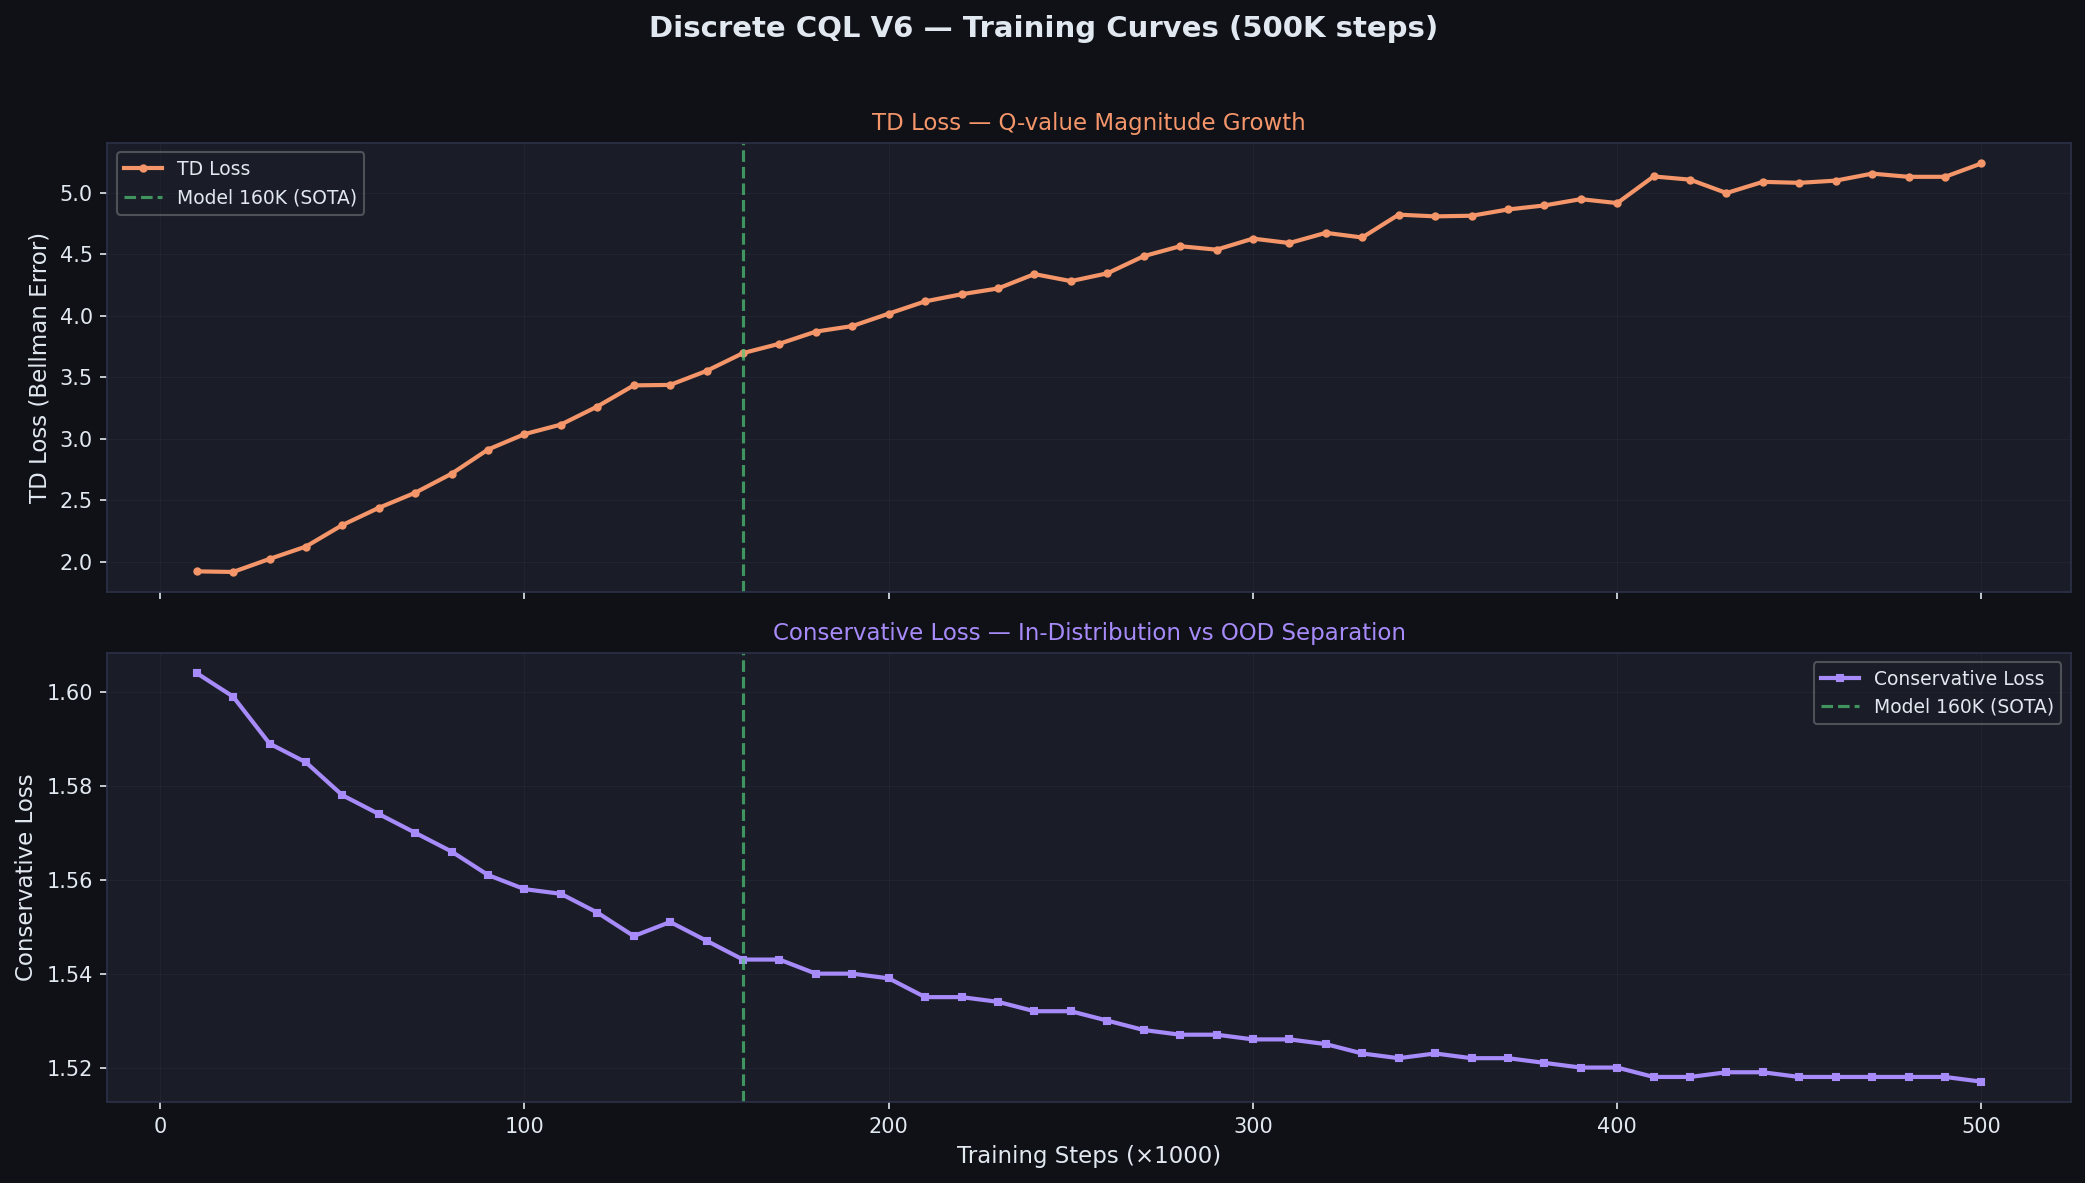
\includegraphics[width=\textwidth]{Images/05_training_curves.png}
    \end{column}
  \end{columns}
\end{frame}

% =====================================================================
% PHẦN 3: KẾT QUẢ
% =====================================================================
\section{Kết quả}

\begin{frame}{Bảng Xếp Hạng Hiệu Năng — 242 Episodes}
  \begin{table}
    \centering
    \begin{tabular}{llccc}
      \toprule
      \textbf{\#} & \textbf{Chiến lược} & \textbf{Gas Cost $\downarrow$} & \textbf{Miss Rate} & \textbf{vs Greedy} \\
      \midrule
      1 & \textbf{Oracle (Hindsight DP)} & \textbf{45,096} & \textbf{0.0\%} & $-$38.8\% \\
      \rowcolor{UTHblue!15}
      2 & \textbf{CQL + Safety 20\%} & \textbf{65,525} & \textbf{0.0\%} & \textbf{$-$11.1\%} \\
      3 & Greedy (Baseline) & 73,710 & 0.0\% & --- \\
      4 & Smart Rule + Safety & 76,892 & 0.0\% & $+$4.3\% \\
      5 & Decision Transformer & $>$100K & 90--100\% & Thất bại \\
      \bottomrule
    \end{tabular}
  \end{table}

  \vspace{0.5em}
  \begin{columns}[T]
    \begin{column}{0.48\textwidth}
      \begin{alertblock}{Kết quả chính}
        Tiết kiệm \textbf{11.1\% Gas} so với Greedy\\
        Miss Rate = \textbf{0.0\%}\\
        Khai thác \textbf{28.6\%} tiềm năng Oracle
      \end{alertblock}
    \end{column}
    \begin{column}{0.48\textwidth}
      \begin{block}{Win Rate}
        CQL thắng Greedy trong \textbf{222/242} episodes\\
        (Win Rate = \textbf{91.7\%})
      \end{block}
    \end{column}
  \end{columns}
\end{frame}

\begin{frame}{Phân tích Chi tiết Từng Episode}
  \centering
  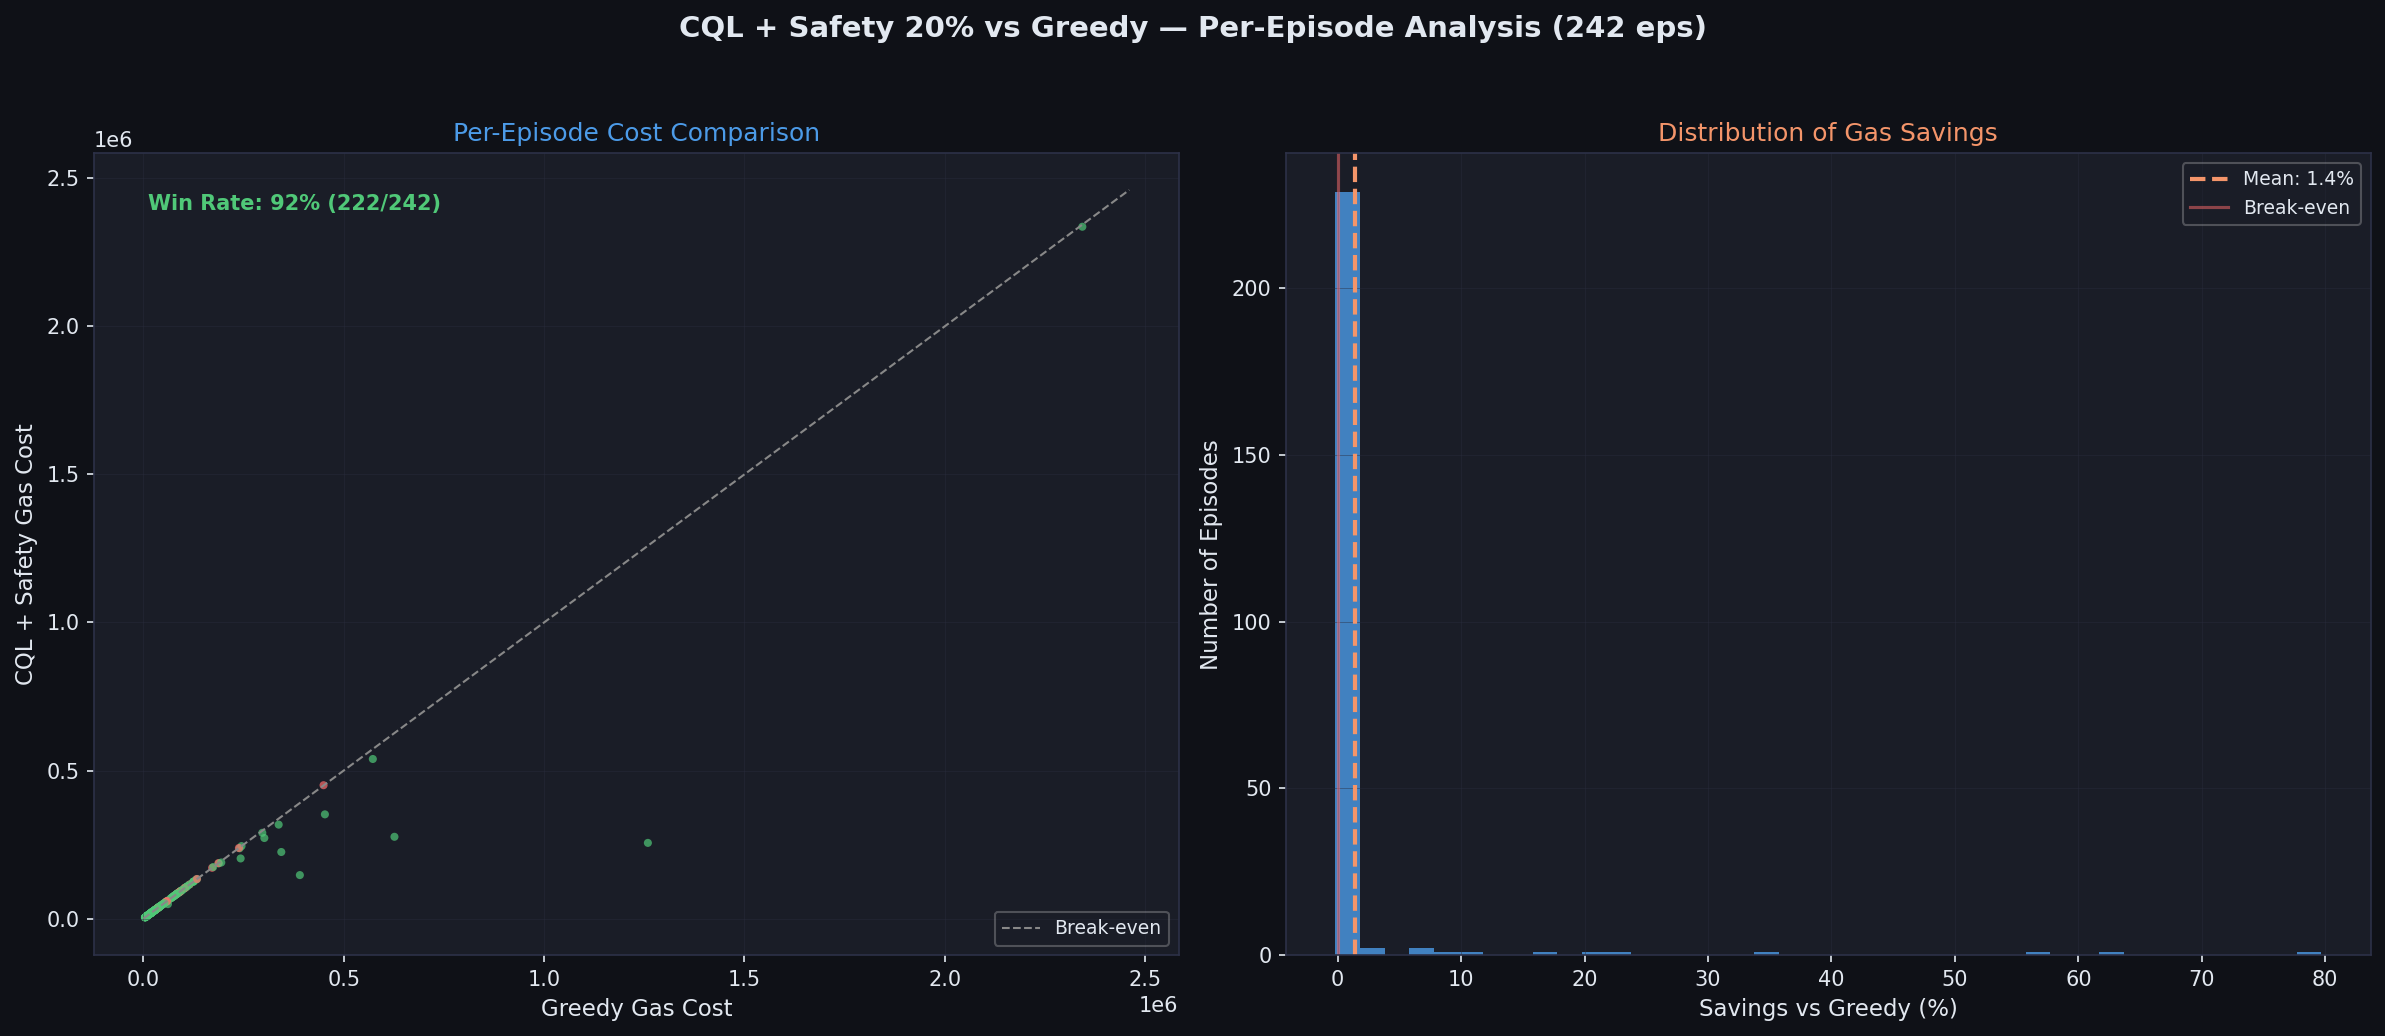
\includegraphics[width=0.88\textwidth]{Images/06_per_episode_comparison.png}
  \vspace{0.5em}

  \begin{columns}[T]
    \begin{column}{0.48\textwidth}
      \begin{itemize}
        \item CQL khai thác cực mạnh ở episodes có Gas biến động lớn (max savings \textbf{79.7\%})
      \end{itemize}
    \end{column}
    \begin{column}{0.48\textwidth}
      \begin{itemize}
        \item Khi CQL thua, mức thua rất nhỏ (tối đa $-$0.2\%) $\Rightarrow$ \textbf{Risk thấp}
      \end{itemize}
    \end{column}
  \end{columns}
\end{frame}

% =====================================================================
% PHẦN 4: PHÂN TÍCH
% =====================================================================
\section{Phân tích}

\begin{frame}{Tại sao Decision Transformer thất bại?}
  \begin{columns}[T]
    \begin{column}{0.48\textwidth}
      \begin{alertblock}{Majority Bias}
        \begin{itemize}
          \item DT học bằng \textbf{Cross-Entropy Loss}
          \item Oracle: Action 0 chiếm \textbf{69.6\%}
          \item DT luôn đoán Action 0 $\Rightarrow$ \textbf{Miss 100\%}
        \end{itemize}
      \end{alertblock}
      \vspace{0.5em}
      \begin{block}{CQL vượt qua nhờ}
        Q-Learning đánh giá \textbf{giá trị thực} của từng hành động, không phụ thuộc vào tần suất
      \end{block}
    \end{column}
    \begin{column}{0.48\textwidth}
      \begin{alertblock}{Risk-Reward Asymmetry}
        \begin{itemize}
          \item Lợi nhuận timing: $O(10^3)$
          \item Hình phạt deadline: $O(10^8)$
          \item Tỷ lệ: \textbf{1 : 223,000}
        \end{itemize}
      \end{alertblock}
      \vspace{0.5em}
      \begin{block}{Reward Shaping giải quyết}
        Giảm penalty $50\times$ (từ 1M $\to$ 20K)\\
        Tăng urgency $3.5\times$\\
        $\Rightarrow$ Agent \textbf{dám khám phá}
      \end{block}
    \end{column}
  \end{columns}
\end{frame}

\begin{frame}[fragile]{Kiến trúc Hệ thống Lai: RL + Safety Layer}
  \centering
  \begin{tikzpicture}[
    box/.style={rectangle, draw=UTHblue, rounded corners=5pt, thick,
      minimum width=3cm, minimum height=1cm, text centered, font=\small},
    arrow/.style={->, very thick, UTHblue},
  ]
    \node[box, fill=UTHblue!15] (input) at (0,0) {$s_t$};
    \node[box, fill=green!15, draw=green!50!black] (ai) at (4.5,1.2) {Discrete CQL};
    \node[box, fill=red!15, draw=red!50!black] (safety) at (4.5,-1.2) {Safety Layer};
    \node[box, fill=UTHgold!30, draw=UTHgold!80!black] (output) at (9,0) {$a_t$};

    \draw[arrow] (input) -- node[above, font=\scriptsize] {$\tau_t > 20\%$} (ai);
    \draw[arrow] (input) -- node[below, font=\scriptsize] {$\tau_t \leq 20\%$} (safety);
    \draw[arrow, green!50!black] (ai) -- node[above, font=\scriptsize] {Tối ưu} (output);
    \draw[arrow, red!50!black] (safety) -- node[below, font=\scriptsize] {Ép xả 100\%} (output);
  \end{tikzpicture}

  \vspace{1em}
  \begin{columns}[T]
    \begin{column}{0.48\textwidth}
      \begin{block}{80\% thời gian đầu}
        AI ``lướt sóng'' giá gas\\
        Tiết kiệm tối đa chi phí
      \end{block}
    \end{column}
    \begin{column}{0.48\textwidth}
      \begin{block}{20\% thời gian cuối}
        Safety Layer ép bán hết\\
        Đảm bảo \textbf{0\% Miss Rate}
      \end{block}
    \end{column}
  \end{columns}

  \vspace{0.5em}
  \centering
  \textit{Đánh đổi: 22.4\% $\to$ 11.1\% savings, nhưng Miss Rate: 0.4\% $\to$ \textbf{0.0\%}}
\end{frame}

% =====================================================================
% PHẦN 5: KẾT LUẬN
% =====================================================================
\section{Kết luận}

\begin{frame}{Kết luận}
  \begin{enumerate}
    \item \textbf{Reward Shaping là chìa khóa:}
    Giảm penalty $50\times$ giúp Agent vượt qua Pessimistic Collapse

    \item \textbf{Data Coverage quyết định:}
    Sự khác biệt nhỏ về Queue Coverage thay đổi hiệu năng tới 40\%

    \item \textbf{Hệ thống Lai = Chuẩn mực thực tiễn:}
    AI 80\% + Safety 20\% $\Rightarrow$ Cân bằng Optimality \& Reliability

    \item \textbf{Hiệu năng vượt trội:}
    \textbf{11.1\% savings}, \textbf{0\% Miss}, Win Rate \textbf{91.7\%}
  \end{enumerate}

  \vspace{1em}
  \begin{block}{Hướng phát triển}
    \begin{itemize}
      \item Tích hợp cấu trúc EIP-1559 (Base Fee + Priority Fee)
      \item Continuous Oracle $\Rightarrow$ Trần tối ưu sâu hơn
      \item LSTM/Transformer dự báo chuỗi thời gian
    \end{itemize}
  \end{block}
\end{frame}

\begin{frame}[plain]
  \centering
  \vspace{3cm}
  {\Huge\textbf{Thank you!}}\\[1em]
  {\Large Kính mời Cô và các bạn đặt câu hỏi}\\[2em]
  % {\normalsize Nguyễn Tiến Duy — 079205037141}
\end{frame}

% =====================================================================
% BACKUP SLIDES
% =====================================================================
\appendix

\begin{frame}{Backup: Tại sao n\_critics = 1?}
  \begin{block}{Double Q-Learning (n\_critics = 2)}
    \begin{itemize}
      \item Dùng $\min(Q_1, Q_2)$ để chống \textbf{Overestimation Bias}
      \item Cần thiết trong Online RL (SAC, TD3)
    \end{itemize}
  \end{block}

  \begin{alertblock}{Nhưng CQL đã có Conservative Penalty!}
    \begin{itemize}
      \item CQL đã chủ động \textbf{đè Q-value xuống} (Underestimate)
      \item Nếu dùng thêm Double Q $\Rightarrow$ \textbf{bi quan kép} (Double Pessimism)
      \item Hậu quả: Q-value $\to -\infty$ $\Rightarrow$ \textbf{Pessimistic Collapse}
      \item Agent sợ hãi, chỉ chọn Action 0 (giữ hàng mãi)
    \end{itemize}
  \end{alertblock}

  \begin{block}{Kết luận}
    \texttt{n\_critics = 1} là lựa chọn \textbf{có chủ ý}, không phải thiếu sót.
  \end{block}
\end{frame}

\begin{frame}{Backup: Backlog Pressure — Mô hình AR}
  \begin{block}{Công thức}
    $b_t = \max(0, \; \rho \cdot b_{t-1} + \alpha_b \cdot p_t + \beta_b \cdot u_t)$
  \end{block}

  \begin{itemize}
    \item \textbf{Autoregressive (AR):} $b_t$ phụ thuộc vào chính $b_{t-1}$ $\Rightarrow$ bộ nhớ ngắn hạn
    \item $\rho = 0.95$: Half-life $\approx$ 14 blocks (phù hợp MEV/NFT drop)
    \item $\alpha_b = 0.3$: Trọng số congestion (gas\_used/target)
    \item $\beta_b = 0.2$: Trọng số transaction surprise
  \end{itemize}

  \begin{block}{Tại sao cần $b_t$?}
    Giúp Agent ``cảm nhận'' sóng tắc nghẽn tích lũy mà \textbf{không cần LSTM/Transformer}
  \end{block}
\end{frame}

\begin{frame}{Backup: Natural Experiment — V6 vs V32}
  \begin{table}
    \centering
    \begin{tabular}{lccc}
      \toprule
      \textbf{Tham số} & \textbf{V33 (Thua)} & \textbf{V32 (Thắng)} & \textbf{Tác động} \\
      \midrule
      \texttt{deadline\_penalty} & 1,000,000 & 20,000 & $50\times$ \\
      \texttt{urgency\_alpha} & 1.0 & 3.5 & $3.5\times$ \\
      \texttt{urgency\_beta} & 0.0001 & 0.0005 & $5\times$ \\
      \texttt{s\_queue} max & 99,006 & 104,135 & Phủ rộng hơn \\
      \midrule
      \textbf{vs Greedy} & Thua 30\%+ & \textbf{Thắng 11.1\%} & \\
      \bottomrule
    \end{tabular}
  \end{table}

  \begin{block}{Bài học}
    \begin{enumerate}
      \item Reward Shaping: Giảm penalty giúp Agent dám khám phá
      \item Data Coverage: Chỉ 5\% chênh lệch queue $\Rightarrow$ thay đổi 40\% hiệu năng
    \end{enumerate}
  \end{block}
\end{frame}

\begin{frame}{Backup: Phân phối Trạng thái}
  \centering
  
\includegraphics[width=0.85\textwidth]{Images/01_state_distributions.png}

  \vspace{0.5em}
  \begin{itemize}
    \item Gas price: Phân phối \textbf{bimodal} (2 chế độ thị trường)
    \item Queue $Q_t$: \textbf{Right-skewed}, max 374K (các cú sốc tắc nghẽn)
  \end{itemize}
\end{frame}

\end{document}
